\documentclass{article}
\usepackage{amsmath,amssymb,graphicx,tikz,pgfplots,booktabs,xcolor}
\pgfplotsset{compat=1.18}

\newenvironment{lesson-meta}{}{}        % lesson code, title, objective, EQ, vocab
\newenvironment{item-analysis}{}{}      % Savvas's Example × DOK table
\newenvironment{model-discuss}{}{}      % Launch opener
\newenvironment{concept-box}{}{}        % in-lesson concept reference
\newenvironment{concept-summary}{}{}    % end-of-lesson summary
\newenvironment{example}[1]{}{}         % #1 = example number
\newenvironment{tryit}[1]{}{}           % #1 = tryit number
\newenvironment{practice}[2]{}{}        % #1 = practice number, #2 = DOK
\newenvironment{te-addendum}[2]{}{}     % #1 = anchor example, #2 = type
\newcommand{\answer}[1]{}               % answer key, inside any env
\newcommand{\placeholder}[2]{}          % #1 = type, #2 = description
\newcommand{\uncertain}[2]{#1}          % #1 = best guess, #2 = alternatives
\newcommand{\te}[1]{}                   % teacher-only inline annotation

\begin{document}

\begin{lesson-meta}
Lesson code: 4-5

Title: Solving Rational Equations

I CAN objective: I CAN\ldots{} solve rational equations and identify extraneous solutions.

Objective: Students will be able to solve rational equations in one variable; identify extraneous solutions to rational equations and give examples of how they arise.

Essential Question: How can you solve rational equations and identify extraneous solutions?

Essential Understanding: Rational equations contain a rational expression and can be solved by multiplying each side of the equation by a common denominator to eliminate the fractions. Any solution that is excluded from the domain of the original equation is extraneous.

Lesson vocabulary: rational equation; extraneous solution.

Topic vocabulary: domain; rational expression; real numbers; undefined.
\end{lesson-meta}

\begin{item-analysis}
\begin{tabular}{lll}
\toprule
Example & Items & DOK \\
\midrule
1 & 15--18, 32 & 1 \\
1 & 12 & 2 \\
2 & 19, 20, 26 & 2 \\
2 & 8 & 3 \\
3 & 21, 22 & 1 \\
3 & 11 & 2 \\
4 & 23, 24, 31 & 1 \\
4 & 10, 14 & 2 \\
4 & 13 & 3 \\
5 & 9, 25, 27--29 & 2 \\
5 & 30, 33 & 3 \\
\bottomrule
\end{tabular}
\end{item-analysis}

\begin{model-discuss}
CRITIQUE \& EXPLAIN

Nicky and Tavon used different methods to solve the equation
\[
\frac{1}{2}x+\frac{2}{5}=\frac{9}{10}.
\]

\begin{tabular}{cc}
\toprule
Nicky & Tavon \\
\midrule
$\frac{1}{2}x+\frac{2}{5}=\frac{9}{10}$ & $\frac{1}{2}x+\frac{2}{5}=\frac{9}{10}$ \\
$\frac{1}{2}x=\frac{9}{10}-\frac{2}{5}$ & $10\left(\frac{1}{2}x+\frac{2}{5}=\frac{9}{10}\right)$ \\
$\frac{1}{2}x=\frac{5}{10}$ & $5x+4=9$ \\
$x=1$ & $5x=5$ \\
The solution is 1. & $x=1$ \\
 & The solution is 1. \\
\bottomrule
\end{tabular}

A. Explain the different strategies that Nicky and Tavon used and the advantages or disadvantages of each.

B. Did Nicky use a correct method to solve the equation? Did Tavon?

C. Use Structure Why might Tavon have chosen to multiply both sides of the equation by 10? Could he have used another number? Explain.

\answer{A. Tavon multiplied the whole equation by 10, which gets rid of the fractions but also adds a step to solving the problem. Nicky kept the fractions, which meant having to find common denominators to do some of the solving. B. Both methods are correct. C. Tavon used 10 because it is the LCD of the fractions. He could have used another multiplier that is a common multiple of the denominators and still gotten a correct answer, but it would mean more reducing.}
\end{model-discuss}

\begin{te-addendum}{ModelDiscuss}{LearnTogether}
Before: Implement Tasks that Promote Reasoning and Problem Solving.

Q: What do you notice about the equation?
\answer{The equation is a linear equation. The coefficient of the $x$-term and the constants are fractions.}
\end{te-addendum}

\begin{te-addendum}{ModelDiscuss}{LearnTogether}
During: Support Productive Struggle in Learning Mathematics.

Q: What strategy does Nicky use to solve the equation?
\answer{Nicky uses a similar strategy as she would use to solve a linear equation with integers. She subtracts to isolate the variable term on one side of the equation; then she divides to isolate the variable.}

Q: What strategy does Tavon use to solve the equation?
\answer{Tavon multiplies each side of the equation by 10. Because each side of the equation is multiplied by the same value, the result is an equivalent equation.}

For Early Finishers:

Q: Solve the equation $\frac{2}{3}x-\frac{4}{5}=1\frac{1}{5}$ using the methods that Nicky and Tavon used. Does each method result in the same solution?
\answer{The solution is $x=3$. Each method of solving this problem results in the same answer.}
\end{te-addendum}

\begin{te-addendum}{ModelDiscuss}{LearnTogether}
After: Facilitate Meaningful Mathematical Discourse.

Q: What do you notice if you rewrite each fraction with a denominator of 10?
\answer{The numerators are the same as those in the equation that Tavon found after multiplying both sides of the equation by 10.}

Q: Substitute $x=1$ into $\frac{1}{2}x+\frac{2}{5}=\frac{9}{10}$ and $5x+4=9$. What does the result tell you about the equations?
\answer{When you substitute $x=1$ in both equations, the equations are true. These are equivalent equations.}
\end{te-addendum}

\begin{te-addendum}{ModelDiscuss}{HabitsOfMind}
Reason If Tavon multiplied each side of the equation by 100, would his answer have been 10 times as much? Explain.
\answer{No; multiplying each side of an equation by the same value does not change the solution of the equation.}
\end{te-addendum}

\begin{concept-box}
Vocabulary: A rational equation is an equation that contains a rational expression.
\end{concept-box}

\begin{example}{1}
Solve a Rational Equation

What is the solution to each rational equation?

A. $\frac{1}{x+4}=2$
\begin{align*}
(x+4)\left(\frac{1}{x+4}\right) &= 2(x+4)\\
1 &= 2x+8\\
x &= -\frac{7}{2}
\end{align*}
The solution is $x=-\frac{7}{2}$.

B. $\frac{1}{x-3}=5$
\begin{align*}
(x-3)\left(\frac{1}{x-3}\right) &= 5(x-3)\\
1 &= 5x-15\\
x &= \frac{16}{5}
\end{align*}
The solution is $x=\frac{16}{5}$.

\answer{A. $x=-\frac{7}{2}$; B. $x=\frac{16}{5}$}
\end{example}

\begin{tryit}{1}
What is the solution to each equation?

A. $\frac{2}{x+5}=4$

B. $\frac{1}{x-7}=2$

\answer{A. $x=-\frac{9}{2}$; B. $x=\frac{15}{2}$}
\end{tryit}

\begin{te-addendum}{1}{LearnTogether}
Establish Mathematics Goals to Focus Learning. Introduce students to rational equations. Remind them that they have added, subtracted, multiplied, and divided rational expressions. This helps students solve rational equations and identify extraneous solutions. Explain that they can use rational equations to solve rate problems.
\end{te-addendum}

\begin{te-addendum}{1}{PurposefulQuestions}
Q: Why do you have to confirm that the solution is valid in the original equation?
\answer{You have to make sure the solution does not cause the denominator of the rational expression to equal zero.}
\end{te-addendum}

\begin{te-addendum}{1}{ElicitEvidence}
Q: Why do you multiply both sides of the equation by the common denominator?
\answer{You multiply both sides by the common denominator to eliminate the fractions.}
\end{te-addendum}

\begin{te-addendum}{1}{HabitsOfMind}
Critique Reasoning For part (b), Kaitlyn wrote $1=2x-7$, then $8=2x$, and $4=x$. Is she correct? Explain.
\answer{No; Kaitlyn did not distribute the 2 properly. The equation becomes $1=2(x-7)$, with $x=7.5$.}
\end{te-addendum}

\begin{example}{2}
Solve a Work-Rate Problem

Arthur and Cheyenne are making Chinese paper cutting designs to give as gifts to wish family and friends good luck in the coming year. Together they can complete the job in 24 hours. How long would it take Cheyenne to complete the job if she was working alone?

\placeholder{illustration}{Arthur and Cheyenne cutting red Chinese paper designs; speech bubble: ``Cheyenne works twice as fast as Arthur.''}

Step 1 Determine the work-rates of Arthur and Cheyenne.

Let $x$ represent the number of hours Arthur needs to finish the job himself.

Arthur works at a rate of
\[
\frac{1\text{ job}}{x\text{ hours}}=\frac{1}{x}\frac{\text{job}}{\text{hour}}.
\]

Cheyenne is twice as fast, so she works at a rate of
\[
\frac{1\text{ job}}{\frac{1}{2}x\text{ hours}}=\frac{2}{x}\frac{\text{jobs}}{\text{hour}}.
\]

Working together, they complete the job in 24 hours, so the work-rate is
\[
\frac{1\text{ job}}{24\text{ hours}}=\frac{1}{24}\frac{\text{job}}{\text{hour}}.
\]

\begin{concept-box}
The amount of a job completed per hour is the work-rate.
\end{concept-box}

Step 2 Write the equation for their rates working together.
\begin{align*}
\frac{1}{x}+\frac{2}{x} &= \frac{1}{24}\\
24x\left(\frac{1}{x}+\frac{2}{x}\right) &= \left(\frac{1}{24}\right)24x\\
24+48 &= x\\
72 &= x
\end{align*}
It takes Arthur 72 hours to create the gifts alone. Since Cheyenne works twice as fast as Arthur, it would take her 36 hours to create the gifts alone.

\answer{36 hours}
\end{example}

\begin{tryit}{2}
It takes 12 hours to fill a pool with two pipes, where the water in one pipe flows three times as fast as the other pipe. How long will it take the slower pipe to fill the pool by itself?
\answer{48 hours}
\end{tryit}

\begin{te-addendum}{2}{PurposefulQuestions}
Q: Why do you add the expressions that represent the two work-rates?
\answer{In one hour, Arthur completes $\frac{1}{x}$ of the job, and Cheyenne completes $\frac{2}{x}$ of the job. Together, they complete $\frac{1}{x}+\frac{2}{x}$ of the job.}

Q: How could you solve this equation without multiplying both sides by $24x$?
\answer{You can add the fractions and then cross-multiply.}
\end{te-addendum}

\begin{te-addendum}{2}{ElicitEvidence}
Q: Why is it important to define the variable before writing an equation to represent the problem?
\answer{Without understanding what the variable represents, it would be difficult to set up the equation correctly.}
\end{te-addendum}

\begin{te-addendum}{2}{CommonError}
You might have multiplied by 2 because Cheyenne works twice as fast. However, it takes Cheyenne half the time to make the gifts.
\end{te-addendum}

\begin{te-addendum}{2}{HabitsOfMind}
Reason In a work-rate problem, explain why you cannot average the individual rates to determine how long it will take to complete a job together.
\answer{Averaging the two rates would result in a rate less than the faster person's rate. But two individuals working together would complete the work in less time than either person with the faster rate could alone.}
\end{te-addendum}

\begin{te-addendum}{2}{RtIExtend}
Use with Example 2. Challenge students to solve a work-rate problem with radical solutions.

Q: Rebecca can rake all of the leaves in a yard in $x$ hours. Angus can rake all of the leaves in a yard in 2 more hours than Rebecca. Together they can rake the yard in 10 hours. How many hours does it take for Rebecca to rake the yard by herself? Write your answer to the nearest hundredth.
\answer{19.05 h}
\end{te-addendum}

\begin{example}{3}
Identify an Extraneous Solution

What is the solution of the equation
\[
\frac{1}{x-5}+\frac{x}{x-3}=\frac{2}{x^2-8x+15}?
\]

Step 1 Multiply each side of the equation by the common denominator, $(x-5)(x-3)$.
\[
(x-5)(x-3)\left(\frac{1}{x-5}+\frac{x}{x-3}\right)=\frac{2(x-5)(x-3)}{x^2-8x+15}
\]

Step 2 Continue to simplify.
\[
\frac{(x-5)(x-3)}{x-5}+\frac{x(x-5)(x-3)}{x-3}=\frac{2(x-5)(x-3)}{x^2-8x+15}
\]

Step 3 Divide out common factors in the numerator and the denominator.
\[
\frac{(x-5)(x-3)}{x-5}+\frac{x(x-5)(x-3)}{x-3}=\frac{2(x-5)(x-3)}{x^2-8x+15}
\]
You can divide out common factors under the assumption that $\frac{x-5}{x-5}=1$ and $\frac{x-3}{x-3}=1$. This is only true if $x\neq5$ or 3.

Step 4 Solve the equation.
\begin{align*}
(x-3)+x(x-5) &= 2\\
x-3+x^2-5x &= 2\\
x^2-4x-3 &= 2\\
x^2-4x-5 &= 0\\
(x-5)(x+1) &= 0\\
x &= 5\text{ and }x=-1
\end{align*}
Consider both solutions. If either solution makes the value of the denominator 0, it is not valid.

The solution $x=5$ is an extraneous solution because it is not in the domain of the original equation.

The solution of the equation $\frac{1}{x-5}+\frac{x}{x-3}=\frac{2}{x^2-8x+15}$ is $-1$.

To see that there is only one solution, graph
\[
f(x)=\frac{1}{x-5}+\frac{x}{x-3}
\quad\text{and}\quad
 g(x)=\frac{2}{x^2-8x+15}.
\]

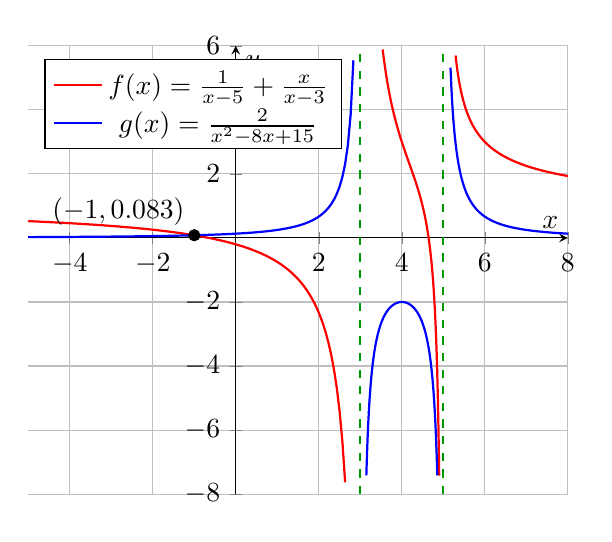
\begin{tikzpicture}
\begin{axis}[
    axis lines=middle,
    xmin=-5, xmax=8,
    ymin=-8, ymax=6,
    xlabel={$x$}, ylabel={$y$},
    xtick={-4,-2,0,2,4,6,8},
    ytick={-8,-6,-4,-2,0,2,4,6},
    grid=both,
    samples=120,
    unbounded coords=jump,
    restrict y to domain=-8:6,
    legend pos=north west
]
\addplot[red, thick, domain=-5:2.9] {1/(x-5)+x/(x-3)};
\addlegendentry{$f(x)=\frac{1}{x-5}+\frac{x}{x-3}$}
\addplot[red, thick, domain=3.1:4.9, forget plot] {1/(x-5)+x/(x-3)};
\addplot[red, thick, domain=5.1:8, forget plot] {1/(x-5)+x/(x-3)};
\addplot[blue, thick, domain=-5:2.9] {2/((x-5)*(x-3))};
\addlegendentry{$g(x)=\frac{2}{x^2-8x+15}$}
\addplot[blue, thick, domain=3.1:4.9, forget plot] {2/((x-5)*(x-3))};
\addplot[blue, thick, domain=5.1:8, forget plot] {2/((x-5)*(x-3))};
\addplot[dashed, green!60!black, thick, forget plot] coordinates {(3,-8) (3,6)};
\addplot[dashed, green!60!black, thick, forget plot] coordinates {(5,-8) (5,6)};
\addplot[only marks, mark=*, black, forget plot] coordinates {(-1,0.083333)};
\node[anchor=south east] at (axis cs:-1,0.083333) {$(-1,0.083)$};
\node[anchor=north] at (axis cs:3,-8) {$x=3$};
\node[anchor=north] at (axis cs:5,-8) {$x=5$};
\end{axis}
\end{tikzpicture}

Both graphs have vertical asymptotes at $x=3$ and $x=5$. Therefore, neither graph has a value at $x=5$. The graphs only intersect in one point, at $x=-1$.

\answer{$x=-1$}
\end{example}

\begin{tryit}{3}
What is the solution to the equation
\[
\frac{1}{x+2}+\frac{1}{x-2}=\frac{4}{(x+2)(x-2)}?
\]
\answer{no solution}
\end{tryit}

\begin{te-addendum}{3}{RtIExtend}
Additional Example 3: What are the solution(s) to the equation
\[
\frac{5}{x+6}+\frac{4}{x+3}=3?
\]
\begin{align*}
(x+6)(x+3)\left(\frac{5}{x+6}+\frac{4}{x+3}\right)&=3(x+6)(x+3)\\
5(x+3)+4(x+6)&=3(x+6)(x+3)\\
5x+15+4x+24&=3x^2+27x+54\\
0&=x^2+6x+5\\
0&=(x+1)(x+5)\\
x&=-1\text{ and }x=-5
\end{align*}
Both $-1$ and $-5$ are in the domain of the original equation, so the solutions are $x=-1$ and $x=-5$.
\end{te-addendum}

\begin{te-addendum}{3}{PurposefulQuestions}
Q: Does a rational equation with multiple solutions always have an extraneous solution?
\answer{No, it is possible that each solution is in the domain of the original equation.}
\end{te-addendum}

\begin{te-addendum}{3}{GeneralizeETP}
Use and Connect Mathematical Representations.

Q: How do you know that the common denominator $(x-5)(x-3)$ will divide out $x^2-8x+15$?
\answer{The product of $x-5$ and $x-3$ is equal to $x^2-8x+15$.}

Q: Are all values that make the value of the denominator 0 extraneous solutions?
\answer{No; in this equation, 3 is a value that makes the denominator 0, but is not an extraneous solution of the equation.}
\end{te-addendum}

\begin{te-addendum}{3}{ElicitEvidence}
Q: How can you use a graph to verify your solution?
\answer{Graph each side of the equation. Notice that the two graphs do not intersect. Therefore, there is no solution.}
\end{te-addendum}

\begin{te-addendum}{3}{ELLAddendum}
Use with Example 3.

Beginning / Speaking: Tell students that this example is about identifying extraneous solutions to equations. Ask students to guess the meaning of extraneous and then use the word to describe things they might see around the classroom that could be viewed as extraneous.

Q: What smaller word do you see at the beginning of the word extraneous?
\answer{extra}

Q: What do you think extraneous means based on what you know about what extra means?
\answer{something extra that is not needed or useful}

Developing / Listening: Read the information in the call-out for Step 3 aloud to students. Have students listen carefully to the usage of the phrase under the assumption. If necessary, have students listen to one example using this phrase to help them understand its meaning more clearly.

Q: What is an assumption?
\answer{something that is accepted as true}

Q: What kind of information would you typically expect to get from a phrase using the word under? Is that how it is used here?
\answer{information about the position or location of an object; no}

Expanding / Writing: Read the call-out for Step 4 with the students. Have students write in their journals the meaning of the term valid, as well as sentences using the term valid.

Q: When is a solution valid?
\answer{A solution is valid when it does not make the denominator of a fraction equal to 0.}

Q: What does not valid mean?
\answer{not reasonable or acceptable}
\end{te-addendum}

\begin{example}{4}
Check for Extraneous Solutions

What are the solutions to the following equations?

A. $\frac{5x}{x-2}=7+\frac{10}{x-2}$
\begin{align*}
\frac{5x}{x-2} &= 7+\frac{10}{x-2}\\
(x-2)\left(\frac{5x}{x-2}\right) &= \left(7+\frac{10}{x-2}\right)(x-2)\\
5x &= 7(x-2)+10\\
5x &= 7x-14+10\\
-2x &= -4\\
x &= 2
\end{align*}
Check the solution in the original equation. The value 2 is an extraneous solution because it would cause the denominator in the original equation to be equal to 0.

This equation has no solution.

B. $\frac{3}{x-3}=\frac{x}{x-3}-\frac{x}{4}$
\begin{align*}
\frac{3}{x-3} &= \frac{x}{x-3}-\frac{x}{4}\\
(4)(x-3)\left(\frac{3}{x-3}\right) &= \left(\frac{x}{x-3}-\frac{x}{4}\right)(4)(x-3)\\
4(3) &= 4(x)-x(x-3)\\
12 &= 4x-x^2+3x\\
x^2-7x+12 &= 0\\
(x-3)(x-4)&=0\\
x-3&=0\text{ or }x-4=0\\
x&=3\text{ or }x=4
\end{align*}
Check the solutions in the original equation. The value 3 is an extraneous solution because it would cause the denominator of the original equation to equal zero. The only solution to the equation is $x=4$.

\answer{A. no solution; B. $x=4$}
\end{example}

\begin{tryit}{4}
What are the solutions to the following equations?

A. $x+\frac{6}{x-3}=\frac{2x}{x-3}$

B. $\frac{x^2}{x+5}=\frac{25}{x+5}$

\answer{A. $x=2$; B. $x=5$}
\end{tryit}

\begin{te-addendum}{4}{PurposefulQuestions}
Q: How can you determine values that cannot be solutions to the equation without solving?
\answer{Any value that makes a denominator zero cannot be a solution to the equation. You can set each denominator equal to zero to find these values.}

Q: Do you have to multiply both sides of the equation by the least common denominator to eliminate the fractions?
\answer{You do not have to multiply by the least common denominator, but you do have to multiply by a common denominator.}
\end{te-addendum}

\begin{te-addendum}{4}{HabitsOfMind}
Have a Growth Mindset: Give Your Best Effort and Persist. When you give your best effort and persist, you have a better chance of reaching your goal. Ask: What does it mean to persist? How do you know that you are getting better at something? How do you feel when you try hard and get better at something?
\end{te-addendum}

\begin{te-addendum}{4}{ElicitEvidence}
Q: What do you notice about the equation in part (b)? How can this help you solve the problem?
\answer{The denominators on each side of the equation are equal. Because the denominators are equal, you can set the numerators equal to each other to solve. Then check for extraneous solutions.}
\end{te-addendum}

\begin{te-addendum}{4}{HabitsOfMind}
Communicate Precisely What is an extraneous solution?
\answer{An extraneous solution is a solution that arises from manipulations of equivalent equations but is not a solution to the original problem.}
\end{te-addendum}

\begin{te-addendum}{4}{RtISupport}
Use with Example 4. Students may need additional practice with multiplying rational expressions, when solving problems with extraneous solutions. Have students practice multiplying these rational expressions.

Find the product.
\begin{align*}
1.\quad &\frac{x-4}{x+7}\cdot\frac{x+5}{x-4}=\frac{x+5}{x+7}\\
2.\quad &\frac{x^2-16}{x^2+6x+9}\cdot\frac{x^2+5x+6}{x^2-3x-4}=\frac{(x+4)(x+2)}{(x+3)(x+1)}\\
3.\quad &\frac{x^2+5x-14}{2x^2+7x-4}\cdot\frac{2x^2-9x+4}{x^2+9x+14}=\frac{(x-2)(x-4)}{(x+2)(x+4)}
\end{align*}
\end{te-addendum}

\begin{example}{5}
Solve a Rate Problem

Paddling with the current in a river, Jake traveled 16 miles. Even though he paddled upstream for an hour longer than the amount of time he paddled downstream, Jake could only travel 6 miles against the current. In still water, Jake paddles at a rate of 5 mph. What is the speed of the current in the river?

\placeholder{illustration}{River scene with canoe; labels ``16 miles downstream'' and ``6 miles upstream.''}

Let $c$ be the rate of the river's current in miles per hour.

Recall that distance $=$ rate $\cdot$ time, so time $=\frac{\text{distance}}{\text{rate}}$.

\begin{concept-box}
Jake's paddle rate in still water $+$ the rate of the current: $5+c$. Jake's paddle rate in still water $-$ the rate of the current: $5-c$.
\end{concept-box}

\[
\frac{16}{5+c}+1=\frac{6}{5-c}
\]
Jake paddles 1 h longer upstream than downstream.

Solve the equation for $c$.
\begin{align*}
\frac{16}{5+c}+1 &= \frac{6}{5-c}\\
(5+c)(5-c)\left(\frac{16}{5+c}+1\right) &= \left(\frac{6}{5-c}\right)(5+c)(5-c)\\
80-16c+25-c^2 &= 30+6c\\
0 &= c^2+22c-75\\
0 &= (c+25)(c-3)\\
0 &= c+25\quad 0=c-3\\
c&=-25\quad c=3
\end{align*}
The solution $c=-25$ is extraneous because the speed of the current cannot be negative.

The speed of the current is 3 mph.

\answer{3 mph}
\end{example}

\begin{tryit}{5}
Three people are planting tomatoes in a community garden. Marta takes 50 minutes to plant the garden alone, Benito takes $x$ minutes and Tyler takes $x+15$ minutes. If the three of them take 20 minutes to finish the garden, how long would it have taken Tyler alone?
\answer{75 minutes}
\end{tryit}

\begin{te-addendum}{5}{RtIExtend}
Additional Example 5. Extend students' understanding by relating the rates people take to complete a task to rational expressions.

Q: What do the rational expressions in the original equation represent?
\answer{$\frac{1}{40}$, $\frac{1}{x-5}$, and $\frac{1}{x}$ represent individual rates to wash a car, and $\frac{1}{20}$ represents the rate for all three to wash a car together.}
\end{te-addendum}

\begin{te-addendum}{5}{PurposefulQuestions}
Q: What does each side of the equation represent?
\answer{the amount of time Jake paddled in one direction}

Q: Why is the 1 added to $\frac{16}{5+c}$ rather than to $\frac{6}{5-c}$?
\answer{$\frac{6}{5-c}$ represents Jake's time traveling upstream, and his time traveling upstream equals 1 hour more than his time traveling downstream.}

Q: Would $c=-25$ be an extraneous solution if you were solving the problem without context?
\answer{No; $c=-25$ would not be an extraneous solution. This solution satisfies the original equation and does not cause the original equation to have a zero in the denominator.}
\end{te-addendum}

\begin{te-addendum}{5}{ElicitEvidence}
Q: How would you set up an equation to solve this problem?
\answer{You know that it takes 20 minutes for three people working together to plant the garden. You can add each person's rate and set it equal to the rate of the three people together.}
\end{te-addendum}

\begin{te-addendum}{5}{CommonError}
Try It 5 Some students may answer the question with the solution of the equation instead of using the solution to answer the question. Emphasize that $x=60$ is the number of minutes it takes Benito to plant the garden on his own, not Tyler. Point out that Tyler takes $x+15$, or 75 minutes. Remind students to make sure that they answer the question being asked.
\end{te-addendum}

\begin{te-addendum}{5}{HabitsOfMind}
Make Sense and Persevere What does the fraction $\frac{1}{50}$ mean with regards to Marta?
\answer{This fraction refers to the amount of garden Marta can plant in 1 minute.}
\end{te-addendum}

\begin{concept-summary}
CONCEPT SUMMARY Solving Rational Equations

WORDS: A rational equation is an equation that contains a rational expression. To solve, identify the domain for the variable. Then multiply both sides of the equation by a common denominator and solve. An extraneous solution is a solution that is not valid because that value is excluded from the domain of the original equation.

ALGEBRA:
\[
\frac{1}{x}+\frac{2}{x}=\frac{1}{6}\qquad\text{Domain: }x\neq0
\]
\begin{align*}
6x\left(\frac{1}{x}+\frac{2}{x}\right)&=6x\left(\frac{1}{6}\right)\\
6+12&=x\\
18&=x
\end{align*}
The domain includes $x=18$, so the solution to the equation is 18.

\[
\frac{x^2+4}{x-1}=\frac{5}{x-1}\qquad\text{Domain: }x\neq1
\]
\begin{align*}
(x-1)\left(\frac{x^2+4}{x-1}\right)&=(x-1)\left(\frac{5}{x-1}\right)\\
x^2+4&=5\\
x^2&=1\\
x&=\pm1
\end{align*}
The domain does not include $x=1$, so 1 is an extraneous solution. It does include $x=-1$, so the solution to the equation is $-1$.

Do You UNDERSTAND?

1. Essential Question How can you solve rational equations and identify extraneous solutions?
\answer{Begin by finding the LCD of all the terms, then multiply each term by the LCD, then simplify. Lastly, substitute the solution into the original equation to see if any of the terms are undefined as a result. If so, that solution cannot be an element of the domain and is considered extraneous.}

2. Vocabulary Write your own example of a rational equation that, when solved, has at least one extraneous solution.
\answer{Sample: $\frac{2}{x+1}-\frac{1}{x-1}=\frac{-2}{x^2-1}$}

3. Error Analysis A student solved the rational equation as follows:
\[
\frac{1}{2x}-\frac{2}{5x}=\frac{1}{10x}-3;\quad x=0
\]
Describe and correct the error the student made.
\answer{The student did not ensure that the solution is valid. This solution is extraneous, and there is no solution to the equation.}

4. Construct Arguments Yuki says, ``You can check the solution(s) of rational equations in any of the steps of the solution process.'' Explain why her reasoning is incorrect.
\answer{Once the original equation has been multiplied by the LCD, the solution might yield values that are not solutions to the original equation.}

Do You KNOW HOW?

Solve.

5. $\frac{4}{x+6}=2$
\answer{$x=-4$}

6. $\frac{x^2}{x+3}=\frac{9}{x+3}$
\answer{$x=3$}

7. Organizing given information into a table can be helpful when solving rate problems. Use this table to solve the following problem.

\begin{tabular}{llll}
\toprule
 & Distance & Rate & Time \\
\midrule
Upstream & & & \\
Downstream & & & \\
\bottomrule
\end{tabular}

A boat can travel 6 km upstream in the same time it takes to travel 12 km downstream. Find the speed of the boat in still water.

\placeholder{map}{Boat traveling between two bridges; labels ``River Current = 4 km/h,'' ``Upstream: 6 km,'' and ``Downstream: 12 km.''}

\answer{12 km/h}
\end{concept-summary}

\begin{te-addendum}{ConceptSummary}{ElicitEvidence}
Q: How can you determine if a solution is in the domain?
\answer{Substitute the solution into the original equation. The solution is in the domain when the denominators are nonzero and the equation is true.}
\end{te-addendum}

\begin{te-addendum}{ConceptSummary}{CommonError}
Exercise 6 Some students may say that the solutions to this equation are $x=3$ and $x=-3$. Have students verify that each solution satisfies the original equation and does not cause the denominator to equal zero.
\end{te-addendum}

\begin{practice}{8}{3}
Reason If you solve a work-rate problem and your solution, which represents the amount of time it would take working together, exceeds the individual working alone times that are given, then how do you know your solution is unreasonable? Explain.
\answer{The time it takes working combined should be less than any of the individual times.}
\end{practice}

\begin{practice}{9}{2}
Construct Arguments Explain why a negative solution must be eliminated as an extraneous solution when solving a rational equation for an unknown rate.
\answer{The rate must be positive.}
\end{practice}

\begin{practice}{10}{2}
Error Analysis Describe and correct the error Miranda made in solving the rational equation.
\[
\frac{1}{x-2}+\frac{x-2}{x+2}=\frac{x-4}{x-2}
\]
Miranda's work:
\begin{align*}
(x+2)(x-2)\left(\frac{1}{x-2}+\frac{x-2}{x+2}\right)&=\left(\frac{x-4}{x-2}\right)(x+2)(x-2)\\
(x+2)(1)+(x-2)(x-2)&=(x+4)(x+2)\\
x+2+x^2-4x+4&=x^2+6x+8\\
-3x+6&=6x+8\\
-2&=9x;\quad x=-\frac{2}{9}
\end{align*}
\answer{In the third step of her work, she incorrectly uses $x+4$ rather than $x-4$ on the right-hand side of the equation. This throws every step thereafter; therefore, the solution is incorrect.}
\end{practice}

\begin{practice}{11}{2}
Generalize In addition to identifying extraneous solutions, why else is it important to substitute your solution into the original equation?
\answer{Verify that students' answers are correct.}
\end{practice}

\begin{practice}{12}{2}
Mathematical Connections Explain how solving rational equations is related to solving linear and quadratic equations.
\answer{Oftentimes the steps involved in solving a rational equation transform it into a linear or quadratic equation.}
\end{practice}

\begin{practice}{13}{3}
Higher Order Thinking Write a rational equation that cannot have 2 or $-6$ as solutions.
\answer{Sample: $\frac{1}{x-2}+\frac{2}{x+6}=10$}
\end{practice}

\begin{practice}{14}{2}
Make Sense and Persevere Solve the rational equation shown. Explain what is unique about the solution.
\[
\frac{x^2-7x-18}{x+2}=x-9
\]
\answer{Sample: The equation reduces to an identity; the solution is the set of all real numbers except $-2$.}
\end{practice}

\begin{practice}{15}{1}
Solve the equation. See Example 1.
\[
\frac{1}{x-3}=10
\]
\answer{$x=\frac{31}{10}$}
\end{practice}

\begin{practice}{16}{1}
Solve the equation. See Example 1.
\[
\frac{15}{x+3}=3
\]
\answer{$x=2$}
\end{practice}

\begin{practice}{17}{1}
Solve the equation. See Example 1.
\[
\frac{12}{x-4}=9
\]
\answer{$x=\frac{16}{3}$}
\end{practice}

\begin{practice}{18}{1}
Solve the equation. See Example 1.
\[
\frac{5}{3-x}=1
\]
\answer{$x=-2$}
\end{practice}

\begin{practice}{19}{2}
Solve the problem. See Example 2.

Working individually, Paige and Malia can each complete a landscaping job in the time shown. Working together, how long would it take them to complete the job?

\placeholder{illustration}{Landscaping scene with two workers; labels ``Malia 4 hours'' and ``Paige 6 hours.''}
\answer{$2\frac{2}{5}$ hours}
\end{practice}

\begin{practice}{20}{2}
Russell and Aaron can build a shed in the time shown when working together. Aaron works three times as fast as Russell. How long would it take Russell to build the shed if he were to work alone?

\placeholder{illustration}{Shed construction scene; speech bubble: ``Russell and Aaron can build the shed in 8 hours working together.''}
\answer{32 hours}
\end{practice}

\begin{practice}{21}{1}
Solve the equation. See Example 3.
\[
\frac{x}{x-3}-4=\frac{3}{x-3}
\]
\answer{no solution}
\end{practice}

\begin{practice}{22}{1}
Solve the equation. See Example 3.
\[
\frac{x^2}{x-10}=\frac{100}{x-10}-10
\]
\answer{$x=-20$}
\end{practice}

\begin{practice}{23}{1}
Solve the equation. See Example 4.
\[
\frac{4}{3(x+1)}=\frac{12}{x^2-1}
\]
\answer{$x=10$}
\end{practice}

\begin{practice}{24}{1}
Solve the equation. See Example 4.
\[
\frac{x}{x-3}+\frac{2x}{x+3}=\frac{18}{(x+3)(x-3)}
\]
\answer{$x=-2$}
\end{practice}

\begin{practice}{25}{2}
Solve the problem. See Example 5.

A boat travels 8 miles upstream in the same amount of time it can travel 12 miles downstream. In still water the speed of the boat is 5 mi/h. What is the speed of the current?
\answer{The speed of the current is 1 mi/h.}
\end{practice}

\begin{practice}{26}{2}
Make Sense and Persevere Kenji can finish a puzzle in 2 hours working alone. Oscar can finish the same puzzle in 3 hours working alone. How long would it take Oscar and Kenji to finish the puzzle if they worked on it together?
\answer{$1\frac{1}{5}$ h}
\end{practice}

\begin{practice}{27}{2}
Use Structure A commercial jet flies 1,500 miles with the wind. In the same amount of time it can fly 1,000 miles against the wind. The speed of the jet in still air is 550 mph. Find the speed of the wind.

\placeholder{illustration}{Wind sock and jet; labels ``Wind Direction'' and ``1,000 miles.''}

a. Organize the given information and what you need to find in a table.

b. Write and solve a rational equation to find the wind speed.

\answer{a. \begin{tabular}{llll}\toprule & Distance & Rate & Time \\\midrule With Wind & 1500 & $550+r$ & $\frac{1500}{550+r}$ \\ Against Wind & 1000 & $550-r$ & $\frac{1000}{550-r}$ \\\bottomrule\end{tabular}

b. $\frac{1500}{550+r}=\frac{1000}{550-r};\ r=110\text{ mi/h}$}
\end{practice}

\begin{practice}{28}{2}
Reason During their day at the beach, Jae and his friends rent a Jet Ski. They split the \$120 rental fee evenly among themselves. Then Jae, with only his friend Orion, share the cost of a \$16 pizza. If Jae spends a total of \$48 for both, then find the number of friends, $n$, with whom he shared the cost of the Jet Ski rental.
\answer{$n=2$ friends}
\end{practice}

\begin{practice}{29}{2}
Make Sense and Persevere When driving to their family reunion, Rio's mom drove 10 miles at a rate of $x$ mph and then 25 miles at a rate of $x+10$ mph. The total driving time was 45 minutes. What were the two driving speeds at which Rio's mom drove?
\answer{40 and 50 mi/h}
\end{practice}

\begin{practice}{30}{3}
Generalize So far this baseball season, Philip has gotten a hit 8 times out of 40 at-bats. He wants to increase his batting average to 0.333. Calculate the number of consecutive hits, $h$, he would need in order to achieve this goal. Round your answer to the nearest whole number.
\answer{$h=8$ hits}
\end{practice}

\begin{practice}{31}{1}
Which of the following rational equations have at least one extraneous solution? Select all that apply.

\begin{tabular}{ll}
$\square$ & $\frac{2}{x}=\frac{3}{x-4}$ \\
$\square$ & $\frac{x^2}{x-3}=\frac{9}{x-3}$ \\
$\square$ & $\frac{x-1}{x-5}=\frac{9}{x-5}$ \\
$\square$ & $x+\frac{3}{x}=4$ \\
$\square$ & $\frac{x}{x-3}-\frac{3}{2}=\frac{3}{x-3}$ \\
\end{tabular}
\answer{$\frac{x^2}{x-3}=\frac{9}{x-3}$ and $\frac{x}{x-3}-\frac{3}{2}=\frac{3}{x-3}$}
\end{practice}

\begin{practice}{32}{1}
SAT/ACT Which of the following is the solution of
\[
\frac{3}{x+1}=\frac{2}{x-3}?
\]

A. $x=-11$\qquad B. $x=-\frac{7}{5}$\qquad C. $x=\frac{7}{5}$\qquad D. $x=11$
\answer{D. $x=11$}
\end{practice}

\begin{practice}{33}{3}
Performance Task A chemist needs alcohol solution in the correct concentration for her experiment. She adds a 6\% alcohol solution to 50 gallons of solution that is 2\% alcohol. The function that represents the percent of alcohol in the resulting solution is
\[
f(x)=\frac{50(0.02)+x(0.06)}{50+x},
\]
where $x$ is the amount of 6\% solution added.

\placeholder{illustration}{Chemist pouring liquid into a container; labels ``x gallons of 6\% alcohol'' and ``50 gallons of 2\% alcohol.''}

Part A How much 6\% solution should be added to create a solution that is 5\% alcohol?

Part B Use Appropriate Tools Explain the steps you could take to use your graphing calculator to verify the correctness of your answer to part (A).

\answer{Part A 150 gallons. Part B Using the graphing function of your calculator, enter $2.5+0.05x$ for $y_1$, and $1+0.06x$ for $y_2$. Then use the TABLE function to find the $y$-values of the functions that are equivalent when $x=150$.}
\end{practice}

\end{document}